\documentclass[10pt,a4paper]{amsart}

\usepackage[]{graphicx}
\usepackage[]{hyperref}
\usepackage[]{physics}
\usepackage[]{listings}
\usepackage[utf8]{inputenc}
\usepackage[toc,page]{appendix}
\usepackage[dvipsnames]{xcolor}

\definecolor{mygray}{gray}{0.9}

\lstset{
	frame = single,
	language = C++,
	showstringspaces = false,
	tabsize = 2,
	otherkeywords = {self},
	keywordstyle = \color{Maroon},
	identifierstyle=\color{olive},
 	stringstyle=\color{orange},
 	backgroundcolor=\color{mygray},
 	breaklines = true
}

\title[Simulation of the Solar System]{The Solar System: an Exercise in Numerical Integration \\
  \hrulefill\small{ FYS3150: Computational Physics }\hrulefill}

\author[Winther-Larsen \& Svalheim]{Sebastian G. Winther-Larsen \\ 
Trygve L. Svalheim \\
\href{https://github.com/gregwinther/FYS3150/}{\texttt{github.com/gregwinther}}}

\date{\today}

\begin{document}

\begin{titlepage}
\begin{abstract}
Two, three, multi. With Euler-Cromer and then Velocity Verlet
\end{abstract}
\maketitle
\tableofcontents
\end{titlepage}

\section{Introduction}

\section{Theory}

\subsection{Newtonian gravtiation}
When one studies the solar system and the way it moves, one inevitably needs to consider the gravity of the situation. The classical law of gravitation is given by Newton's law
\begin{equation}
\label{eq:newtoniangravity}
F_G = \frac{GM_1M_2}{r^2},
\end{equation} 
where $F_G$ is the gravitational force between to bodies, $G$\footnote{$G=6.67408 \times 10^{-11} m^3 kg^{-1} s{-2}$} is the gravitational constant, $M_1$ and $M_2$ are the masses of the two bodies and $r$ is the distance between them.

In three dimensions, by employing Newton's second law of motion, one will get the following componental equations for the acceleration due to gravitational pull on a particular body $i$.
\begin{equation}
\label{eq:componentalnewton}
\frac{d^2x}{dt^2} = \frac{F_{G,x}}{M_i}, \quad
\frac{d^2y}{dt^2} = \frac{F_{G,y}}{M_i}, \quad
\frac{d^2z}{dt^2} = \frac{F_{G,z}}{M_i},
\end{equation}
each of which can be integrated in order to find the position of the bodies at any given time and for a particular inital velocitiy and position. Moreover, a neat vectorial expression for the Newtonian gravity (equation \ref{eq:newtoniangravity}) in three dimensions is
\begin{equation}
\vb{F}_G = \frac{GM_1M_2}{r^3}\vb{r}
\end{equation}
where $\vb{r}$ gives the posistion of the body in a cartesian coordinate system.

\subsection{Relativity}

The theory of general relativity (GR), put forth by Albert Einstein in 1915, is the current description of gravity in modern physics. On curiosity of the solar system that cannot be explained is the perihelion precession of Mercury's orbit. For every Mercury year the perihelion of the planets orbit moves sligthly. The observed value of this effect is $43$ arc-seconds per century. Einstein showed himself that GR could explain this anomaly.

Closed elliptical orbits are a special feature of the factor ($1/r^2$) in Newton's law of gravitation. Any change to this factor will result in a change in the orbit. For a small such correction, each orbit will be almost the same, but as time progresses the orientation of the elliptical orbit will itself rotate. In this study we will not compute a space-time manifold in order to make this correction, but rather add a general relativistic error term to the Newtonian gravitational force (equation \ref{eq:newtoniangravity}.
\begin{equation}
\label{eq:relativenewton}
F_G = \frac{GM_{\odot}M_{Mercury}}{r^2}\left[1+\frac{3l^2}{r^2c^2} \right],
\end{equation}
where $M_{MERCURY}$ is the mass of Mercury, $r$ is the distance between Mercury and the Sun, $l=\abs{\vb{r}\times\vb{v}}$ is the orbital angular momentum per unit mass, and $c$ is the speed of light in vacuum.

\section{Units}
In order to make the system easy to work with and the calculations easier as well, a change of units is warranted. In this study we will therefore express the mass of any body as a fraction of solar masses, that is $M_{\odot} = 2\times10^{30}kg$. This means that the Earth\footnote{In SI-units, $M_{Earth}\approx6\times10^{24}kg$}, for instance will have a mass of $M_{Earth}= 3\times10^{-6}$.

Additionally, the units for distance will be astronmical units $AU$. This is the mean distance between the earth and the sun. For a simple system and a particular coordinate system with the sun at origin, the initial position for the Earth could simply be $\vb{r}_ {Earth}=(1,0,0)$.

The unit for time will be Earth years, $yr$. This means that velocity will be in units $AU/yr$.

Changing the variables will have consequences for the gravitationan constant $G$ and velocities $v$ as well. This can be deduced easily enough by picking a sample system consisting of the earth and the sun. Inserting in equation \ref{eq:newtoniangravity} gives
\begin{equation}
\label{eq:earthandsun}
F_G = \frac{GM_{\odot}M_{Earth}}{r^2}
\end{equation}
Furthermore, assuming the orbit of the earth is perfectly circular, will give the following relation
\begin{equation}
\label{eq:circularearth}
F_G = \frac{M_{Earth}v^2}{r}
\end{equation}
Combining equations \ref{eq:earthandsun} and \ref{eq:circularearth} yields the following
\begin{equation}
v^2r=gM_{\odot}=4\pi^2AU^3yr^{-2}
\end{equation}
Because the mass of the sun as a fraction of solar masses is $M_{\odot}=1$  and the distance between the earth and the sun is $r=1AU$ we land at
\begin{equation}
G=4\pi^2AU^3yr^{-2} \quad v_{Earth}=2\pi AUyr^{-1}
\end{equation}

\section{Algorithms and implementation}

\subsection{Object orientation}
Object orientation allows for more general code to be written and for easy reuse. Moreover, object orientation makes sense for humans, who tends to classify objects we see and interact with in everyday life. In this study we make use of all the advantages of object oriented programming by implementing several classes. A class diagram illustration of the program is included in appendix \ref{app:classdiagram}. Bear in mind that this diagram does not represent the functionality of the program to a full extent, as many methods and a few classes are left out. Rather, it helps one to understand how the class hierarchy is built up and how the program as whole is supposed to function.

The \lstinline|System| class contains all the information about the initial conditions of the system, which integration method should be used and also some helpful methods, like one that writes data to file.

The \lstinline|InitialCondition| superclass contains a method for setting up particles. Depending on what system one wants to model, we have implemented three subclasses of \lstinline|IntialCondition|: \lstinline|TwoBody|, \lstinline|ThreeBody| and \lstinline|MultiBody|. The name of these classes speek mostly for themselves.

The intersting objects, contained within the \lstinline|InitialCondition| subclasses are instances of the \lstinline|Particle| class. The class could have another name, like "planet" or "body" because instances of it will represent the largest bodies in the solar system; the sun and (eventually) all nine planets\footnote{Including Pluto for historical reasons.}. Every particle instance takes a position vector, a velcity vector and a mass as inputs and has only these attributes\footnote{The position and velocity vectors are defined by its own class \lstinline|Vec3|.}. The extra abstraction to "particle" if therefore fitting, and the class could be employed elsewhere, for instance in a molecular dynamics simulation.

The \lstinline|Integrator| superclass har two subclasses \lstinline|EulerCromer| and \lstinline|VelocityVerlet| each of which must owerwrite the \lstinline|integrateOneStep| method. These are the most important part of the program, because it is where the essential part of the two algorithms are implemented. The \lstinline|integrateOneStep| method is called iteratively for a specified number of steps from a class instance of the \lstinline|system| class, hence the name of the method. Within the \lstinline|integrateOneStep| method, the integration is performed for every particle in the system. A further description of the integrator algorithms follows.

\subsection{Euler-Cromer}

Analytically the Euler-Cromer method, or the semi-implicit Euler method, can be expressed in one dimension by the following recursive relations
\begin{align}
v_{n+1} &= v_n + a_n dt \\
x_{n+1} &= x_n + v_{n+1} dt,
\end{align}
where $a_n$ is the acceleration, $v_n$ is the velocity and $x_n$ is the position, after a certain number of steps $n$. $dt$ is the time step and $t_n = t_0 + ndt$ is the time after $n$ steps. One sees that the algorithm is relatively cheap, with $4n$ FLOPS. In C++ code the \lstinline|integrateOneStep| method of the \lstinline|EulerCromer| class looks like this
\begin{lstlisting}
void EulerCromer::integrateOneStep(std::vector<Particle*> particles) {

	m_system->computeForces();
    
	for (int i=0; i<particles.size(); i++) {
		Particle *p = particles.at(i);

		// Acceleration vector
		vec3 a = (p->getForce()) / (p->getMass());
        
		// Velocity update
		p->getVelocity() += m_dt*a;

		// Position update
		p->getPosition() += m_dt*p->getVelocity();
	}
}
\end{lstlisting}
Notice that the forces used to compute the acceleration are computed within the \lstinline|System| class and that the method uses three-dimensional vectors for more realistic results.

The Euler Cromer method is a first-order integrator which means that it commits a global error of the order of $dt$. This means that by decreasing the time step one will get a more accurate result.

\subsection{Velocity Verlet}
The Verlet method is an integration method designed to integrate Newton's equation of motion. The method provides good numerical stability and more precise results compared with a regular method like the Euler-Cromer method. The reason for this is that it is symplectic, which means that it conserves state-space volume\footnote{One would probably read an entire book to understand this, so we will leave it at that.}.

The velocity Verlet method can also be represented by a (one-dimensional) recursive relation
\begin{align}
x_{n+1} &= x_n + v_ndt + \frac{1}{2}a_ndt^2 \\
v_{n+1} &= v_n + \frac{a_n + a_{n+1}}{2}dt.
\end{align}
These equations tell us that the algorithm is slightly more expensive compared to the Euler-Cromer scheme at $11n$. Here follows an implementation of the algorithm in C++.

\begin{lstlisting}
void VelocityVerlet::integrateOneStep(std::vector<Particle*> particles) {
    
	m_system->computeForces();
    
	for (int i=0; i<particles.size(); i++) {
		Particle *p = particles.at(i);

		// Acceleration vector
		vec3 a = (p->getForce()) / (p->getMass());

		// Position update
		p->getPosition() += p->getVelocity()*m_dt + 0.5*a*m_dt*m_dt;

		m_system->computeForces();

		// New accelration vector
		vec3 anew = (p->getForce()) / (p->getMass());

		// Velocity update
		p->getVelocity() += (a + anew)*m_dt/2;
	}
}
\end{lstlisting}
One sees that it is necessary to compute forces and update acceleration once more in order to update the velocity, which means more operations must be conducted. Time will show if the extra cost of this algorithm is worth the  increase in precision it promises.

\section{Data}
As we wish to determine the orbits of our solar system as accurately as possible, we use date from HORIZON Web-Interface, provided by the Jet Propulsion Laboratory (NASA) at the California institute of technology: \url{http://ssd.jpl.nasa.gov/horizons.cgi}. Here of data from several celestial bodies can be downloaded. It is simple to find both position and velocity for all particles in our bodies at high precision. Units of length can be set to $AU$ and velocities to $AU$ per day. The velocities must be converted for our simulation. We have faith that these data are accurate.

\section{Results}

The object-oriented model for the solar system that has been built is very flexible, as the reader will soon come to know. We start by constructing some simple models with two and three bodies, then the entire solar system, and lastly, simulate the perihelion precession of Mercury, as discussed in the theory section.

\subsection{Two-Body system: Earth and Sun}

\begin{figure}[ht]
	\centering
	\textbf{Comparison of Euler-Cromer and Velocity Verlet}
	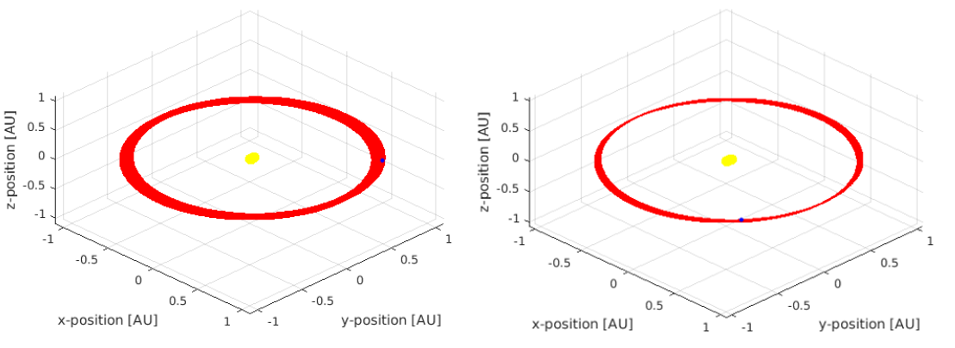
\includegraphics[width=0.99\textwidth]{../figures/earthcompare.png}
	\label{fig:earthcompare}
	\caption{Figure showing the difference in precision between the Euler-Cromer method (left) and the velocity Verlet method (right). The time step is $dt=10^{-2}$ and the number of points is $N=10^6$}
\end{figure}

\begin{figure}[ht]
	\centering
	\textbf{Earth Escape Velocity}
	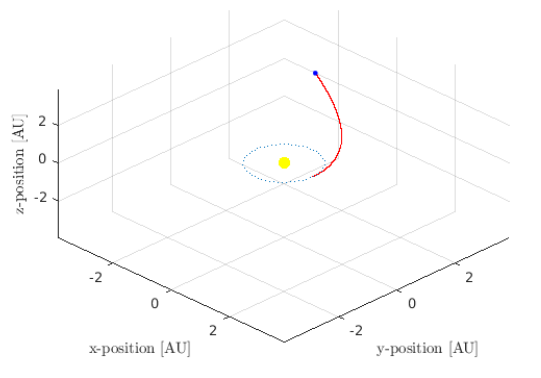
\includegraphics[width=0.9\textwidth]{../figures/earthescape.png}
	\caption{Illustration of Earth escaping orbit at $\sqrt{8}\pi AU/yr$}
\end{figure}


\subsection{Three-Body system: Earth, Sun and Jupiter}

\begin{figure}[ht]
	\centering
	\textbf{Earth, Sun and Jupiter}
	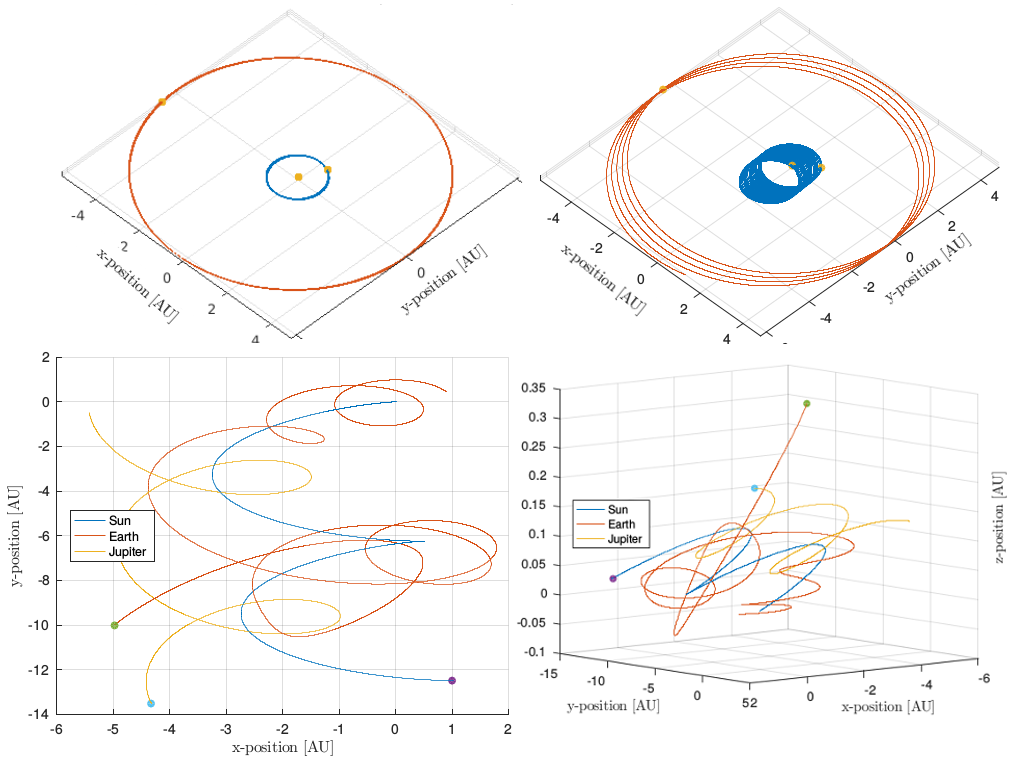
\includegraphics[width=0.99\textwidth]{../figures/threebody.png}
	\caption{Model outcome for a Jupiter with different masses. Top left: Normal mass. Top right: Jupiter mass $10\times$ normal. Bottom: Jupiter mass $1000\times$ normal, in 2D (left) and 3D (right)}
\end{figure}

\subsection{Multi-Body system: all planets}

\subsection{The perihelion precession of Mercury}

\section{Discussion}


\section{Conclusion}

\pagebreak

\begin{appendix}

\section{Class Diagram}
\label{app:classdiagram}

\begin{figure}[ht]
	\centering
	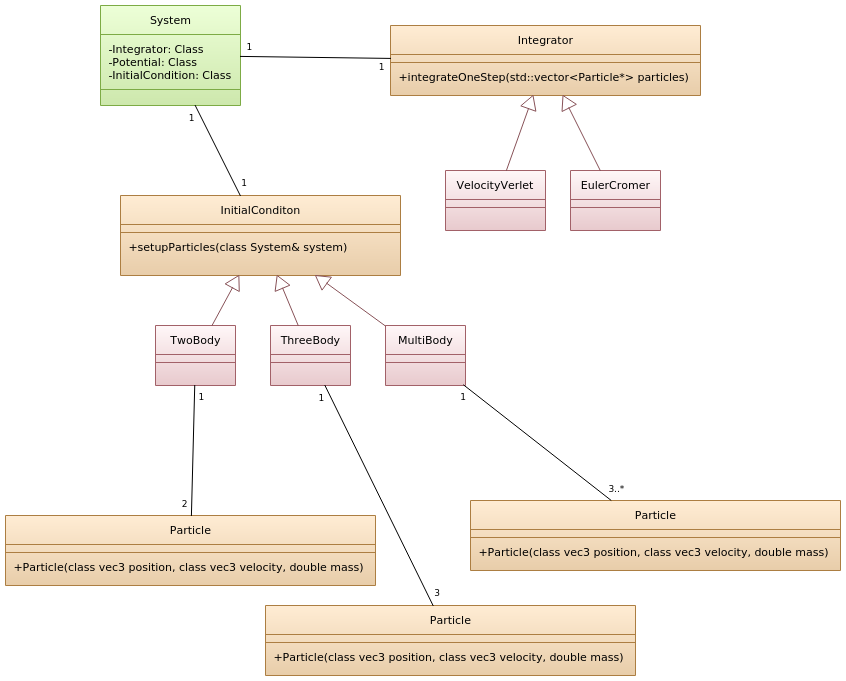
\includegraphics[width=0.9\textwidth]{../figures/classdiagram.png}
\end{figure}

\end{appendix}

\end{document}
